\documentclass[12pt]{article}
\usepackage[utf8]{inputenc}
\usepackage[T1]{fontenc}
\usepackage{mathptmx}
\usepackage{geometry}
\usepackage{mathtools}
\usepackage[english]{babel}
\usepackage{graphicx}
\usepackage[figurename=Gambar]{caption}
\usepackage{hyperref}
\usepackage{minted}
\usepackage{setspace}
\usepackage{color}
\usepackage[explicit]{titlesec}
\usepackage{tocloft}
\usepackage{titletoc}
\usepackage{indentfirst}
\usepackage{caption}
\usepackage{subcaption}
\usepackage{amsmath} 

%\color{white}
%\pagecolor{black}

\hypersetup{colorlinks,
	citecolor=black,
	filecolor=black,
	linkcolor=black,
	urlcolor=black
}

\geometry{
	a4paper,
	left=40mm,
	right=30mm,
	top=20mm,
	bottom=20mm,
}

\date{}

%=============================================================================
% Modified Items

\providecommand{\keywordid}[1]{\textit{Kata Kunci: } #1}
\providecommand{\keyworden}[1]{\textit{Keywords: } #1}

\titleformat{\section}{}{}{0pt}{}
%\titleformat{\subsubsection}{\small \bfseries}{\thesubsection}{0pt}{}

\renewcommand{\cftsecleader}{\cftdotfill{\cftdotsep}}
\renewcommand{\cftsubsecleader}{\cftdotfill{\cftdotsep}}

%\makeatletter
%\let\latexl@section\l@section
%\def\l@section#1#2{\begingroup\let\numberline\@gobble\latexl@section{#1}{#2}\endgroup}
%\makeatother

\addto\captionsenglish{\renewcommand{\contentsname}{}}
\addto\captionsenglish{\renewcommand{\listfigurename}{}}

\renewcommand{\cftsecfont}{\normalfont}
\renewcommand{\cftsecpagefont}{\normalfont}

\renewcommand{\thefigure}{\arabic{section}.\arabic{figure}}

\hyphenation{reposi-tori}

%=============================================================================
% Document Part

\begin{document}
	
%\onehalfspacing

%=============================================================================
% Soft Cover

	\pagenumbering{roman}
%	\setcounter{page}{2}
	
%=============================================================================
%\newpage
%\thispagestyle{plain}
%\mbox{}

%=============================================================================
% Daftar Isi
\newpage

	\begin{center}
		\textbf{{\large Daftar Isi}}
	\end{center}
	
	\tableofcontents

%=============================================================================
%\newpage
%\thispagestyle{plain}
%\mbox{}

%=============================================================================
% Daftar Gambar
\newpage

	\begin{center}
		\textbf{{\large Daftar Gambar}}
	\end{center}

	\listoffigures

%=============================================================================
%\newpage
%\thispagestyle{plain}
%\mbox{}

%=============================================================================
\newpage

	\pagenumbering{arabic}
	\setcounter{page}{3}

	\setcounter{section}{0}
	
	\setcounter{figure}{0}
	
	\setcounter{subsubsection}{0}
	
	\begin{center}
		{\large \textbf{Git Kolaborasi}}
	\end{center}
	
	\section{Kolaborasi}
	
	Bab ini akan membahas secara ringkas bagaimana menggunakan Git dan Github untuk bekerja secara kolaboratif.
	Git dan Github dapat digunakan untuk pengembangan suatu proyek secara kerja sama antar banyak akun Github dengan satu akun sebagai \textit{maintainer}.
	Perlu diperhatikan, pembahasan disini hanya menggunakan metode \textit{pull request} dan \textit{merge} tanpa perlu ada akses \textit{Collaborator} yang disediakan Github.
	Yang dibutuhkan adalah:
	\begin{itemize}
		\item Koneksi internet yang stabil
		\item Github Account
		\item Git client (Linux/Windows), dengan dilengkapi:
		\begin{itemize}
			\item Git Bash atau Bash shell
			\item Git GUI atau Git Cola
		\end{itemize}
	\end{itemize}

	Sebagian besar tahapan-tahapan ini dilakukan di terminal, yang dapat diakses dengan:
	\begin{itemize}
		\item untuk Windows. Klik kanan pada ruang kosong Explorer dan pilih \textbf{Git Bash here}.
		\item untuk Linux. Klik kanan pada ruang kosong File Manager dan pilih \textbf{Open Terminal Here}.  
	\end{itemize}

	\subsection{Persiapan}
	
	Pada tahap ini, dilakukan dua langkah utama, yaitu \textbf{Forking} dan \textbf{Add Upstream}.
	Tahapan ini cukup dilakukan sekali saja untuk satu proyek. 
	
	\subsubsection{Forking}
	
	Forking adalah proses mengambil dan menggandakan suatu proyek repositori, terutama antar akun Github.
	Repositori hasil forking ini akan menjadi acuan dasar untuk pengembangan suatu proyek.
	
	Selanjutnya berikut adalah contoh suatu repositori untuk mempermudah penjelasan:
	\begin{itemize}
		\item user pertama: \textbf{mekatronik-achmadi}
		\begin{itemize}
			\item repositori proyek: \textbf{photsim}
			\item cabang repositori: \textbf{master}	 
		\end{itemize}
		\item user kedua: \textbf{friends} 
	\end{itemize}

	Kemudian berikut langkah mudah forking repositori:
	
	\begin{enumerate}
		\item Buka webbrowser, login akun anda di Github \url{https://github.com/}
		Sebagai contoh disini, akun anda adalah \textbf{friends}
		\item Kunjungi repositori yang akan di forking di Github.
		Sebagai contoh disini adalah repositori sebagaimana di atas, yaitu \url{https://github.com/mekatronik-achmadi/photsim}.
		\item Klik tombol Fork yang ada di pojok kanan atas halaman repositori.
		 
		\begin{figure}[h!]
			\centering
			\captionsetup{justification=centering}
			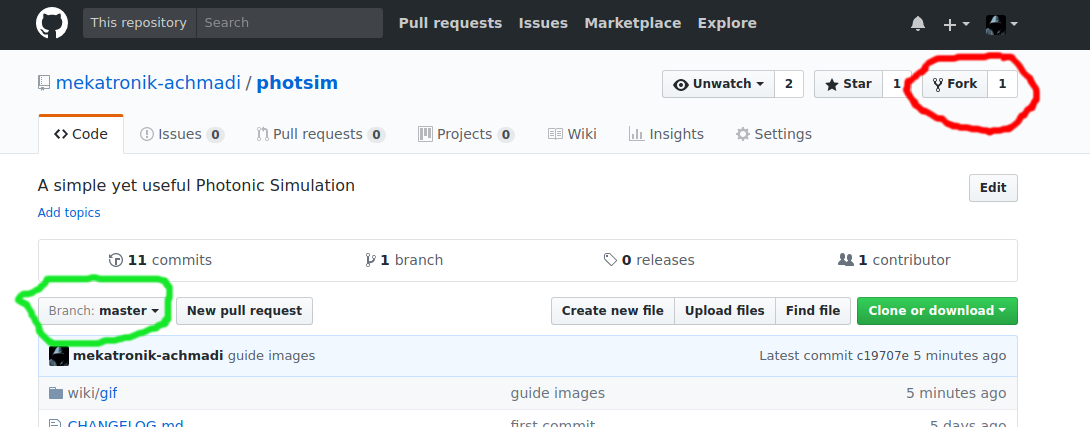
\includegraphics[width=0.8\linewidth]{../images/png/fork_branch}
			\caption[Tombol Fork dan Branch]{\small{Tombol Fork (tanda merah) dan Daftar Branch/Cabang (tanda hijau)}}
		\end{figure}
	
		\item tunggu proses forking selesai, maka kemudian anda memiliki salinan repositori di akun github anda.
	 
	\end{enumerate}
	
	\subsubsection{Add Upstream}
	
	Setelah anda memiliki salinan repositori pada akun Github anda,
	selanjutnya anda perlu membuat salinan lokal di komputer/laptop anda dengan dua alamat remote,
	yaitu akun Github anda sendiri dan akun asal repositori (sebagai \textbf{upstream}).
	
	Berikut adalah langkah-langkah tahapan untuk tahapan ini:
	
	\begin{itemize}
		\item Buka Git Bash (Windows) atau Bash Shell (Linux) pada direktori/folder repositori.
		\item \textit{Clone} repositori di Github anda ke lokal komputer/laptop.
		Sebagai contoh, hasil forking pada tahapan sebelumnya memiliki repositori:
		\begin{itemize}
			\item user name: \textbf{friends}
			\item repositori proyek: \textbf{photsim}
			\item cabang repositori: \textbf{master}
		\end{itemize}
	
		Perintah untuk \textit{clone}:
		\begin{minted}[frame=lines,fontsize=\footnotesize]{bash}
git clone  https://github.com/friends/photsim.git
		\end{minted}
		
		\item Masuk ke folder repositori dan pindah ke cabang/branch \textbf{master}:
		\begin{minted}[frame=lines,fontsize=\footnotesize]{bash}
cd ./photsim
git checkout master
		\end{minted}
		
		\item Selanjutnya, tambahkan repositori asal sebagai \textbf{upstream}.
		Sebagai contoh, pada tahapan sebelumnya repositori asal: 
		\begin{itemize}
			\item user name: \textbf{mekatronik-achmadi}
			\item repositori proyek: \textbf{photsim}
			\item cabang repositori: \textbf{master}
		\end{itemize}
		Perintah untuk tambah \textit{upstream}:
		\begin{minted}[frame=lines,fontsize=\footnotesize]{bash}
git remote add upstream https://github.com/mekatronik-achmadi/photsim.git
		\end{minted}	
	
		\item Terakhir untuk mengecek semua alamat remote:
		\begin{minted}[frame=lines,fontsize=\footnotesize]{bash}
git remote -v
		\end{minted}
	\end{itemize} 

	\subsection{Workflow}
	
	Setelah pada tahapan sebelumnya selesai maka dapat dilanjutkan untuk tahapan \textit{workflow}.
	Tahapan sebelumnya (Persiapan) cukup sekali saja atau bila diperlukan.
	Sedangkan tahapan ini adalah tahapan inti (utama) yang dapat dilakukan berulang-ulang.
	
	Pada tahap ini, dilakukan enam langkah utama, yaitu:
	\begin{itemize}
		\item Update dari Upstream
		\item Buat Branch/Cabang tersendiri
		\item Editing/Development
		\item Upload ke Github sendiri
		\item Pull Request
		\item Hapus Branch/Cabang
	\end{itemize}

	\subsubsection{Update dari Upstream}
	
	Pada langkah ini, dilakukan update atau sinkronisasi repositori anda dengan repositori \textbf{upstream}.
	Langkah sangat penting agar pengembangan anda nantinya sudah berdasarkan versi mutakhir (terupdate).
	Update atau sinkronisasi ini dilakukan baik untuk repositori lokal maupun Github.
	
	Langkah-langkah untuk update dari Upstream:
	
	\begin{itemize}
		\item Buka Git Bash (Windows) atau Bash Shell (Linux) pada direktori/folder repositori.
		
		\item \textit{Fetch} atau ambil update dari \textbf{upstream}
		\begin{minted}[frame=lines,fontsize=\footnotesize]{bash}
git fetch upstream
		\end{minted}
		
		\item Pindah ke branch/cabang \textbf{master}
		\begin{minted}[frame=lines,fontsize=\footnotesize]{bash}
git checkout master
		\end{minted}
		
		\item \textit{Merge} atau satukan antara update \textbf{upstream} dan \textbf{master}
		\begin{minted}[frame=lines,fontsize=\footnotesize]{bash}
git merge upstream/master
		\end{minted}
		
		\item Selanjutnya anda dapat mem-\textit{push} atau upload update ini ke repositori Github anda sendiri
		\begin{minted}[frame=lines,fontsize=\footnotesize]{bash}
git push origin master
		\end{minted}
	\end{itemize}

	\subsubsection{Buat Branch/Cabang tersendiri}
	
	Selanjutnya pada tahapan ini anda dapat membuat cabang/branch baru untuk dapat lakukan editing/development pada proyek anda ini.
	Pada dasarnya, tanpa membuat cabang/branch baru, anda sudah dapat editing/development pada branch \textbf{master}.
	Namun ini sering dinilai tidak layak mengingat branch \textbf{master} adalah branch utama yang harus bersih dari kegiatan uji coba.
	
	Sebagai contoh, disini akan dibuat branch baru \textbf{mybranch}.
	Berikut adalah langkah-langkah membuat branch baru:
	
	\begin{itemize}
		\item Buka Git Bash (Windows) atau Bash Shell (Linux) pada direktori/folder repositori.
		
		\item Buat branch baru bernama \textbf{mybranch}
		\begin{minted}[frame=lines,fontsize=\footnotesize]{bash}
git branch mybranch
		\end{minted}
		
		\item Cek semua branch yang sudah ada
		\begin{minted}[frame=lines,fontsize=\footnotesize]{bash}
git show-branch -a
		\end{minted}
		
		\item Pindah branch ke yang baru
		\begin{minted}[frame=lines,fontsize=\footnotesize]{bash}
git checkout mybranch
		\end{minted}
		
	\end{itemize} 

	\subsubsection{Editing/Development}	
	
	Pada tahapan ini, anda sudah dapat melakukan editing, pengujian, dan semua kegiatan pengembangan proyek.
	Perlu diingat bahwa semua pekerjaan ini hanya dilakukan pada branch \textbf{mybranch}.
	Sedangkan branch \textbf{master} tetap terjaga tidak mengalami perubahan
	
	\subsubsection{Upload ke Github sendiri}
	 
	Selanjutnya, setelah seluruh development selesai anda dapat upload atau \textit{push} hasil kerja anda ke Github anda sendiri.
	Hal-hal yang perlu diperhatikan sebelum anda \textit{push} ke Github:
	
	\begin{itemize}
		\item Pastikan hasil kerja anda bisa diuji ulang oleh \textit{maintainer}.
		\item Pastikan direktori/folder repositori bersih dari file-file hasil kompilasi/\textit{generate}.
		\item Pastikan direktori/folder telah berisi semua dan hanya file-file yang anda kerjakan.
	\end{itemize} 

	Berikut langkah-langkah \textit{push} atau upload ke Github:
	
	\begin{itemize}
		\item Buka Git Bash (Windows) atau Bash Shell (Linux) pada direktori/folder repositori.
		
%=============================================================================
\newpage
		
		\item cek semua file yang akan di commit
		\begin{minted}[frame=lines,fontsize=\footnotesize]{bash}
git status
		\end{minted}
		
		\item Stage semua file yang akan di \textit{commit}.
		\begin{minted}[frame=lines,fontsize=\footnotesize]{bash}
git add -A
		\end{minted}
		
		\item Commit semua hasil pekerjaan
		\begin{minted}[frame=lines,fontsize=\footnotesize]{bash}
git commit -m "my work today"
		\end{minted}
		
		\item \textit{Push} branch hasil kerja ke Github
		\begin{minted}[frame=lines,fontsize=\footnotesize]{bash}
git push -u origin mybranch
		\end{minted}
		
	\end{itemize}

	\subsubsection{Pull Request}
	
	Setelah tahapan \textit{push}, selanjutnya anda dapat membuat \textit{Pull Request}.
	\textbf{Pull Request} adalah permintaan yang anda ajukan kepada akun Github \textit{maintainer} yang berisi \textit{patch} atau modifikasi/perubahan dari hasil kerja anda.
	Perlu diingat kembali, bahwa \textit{pull request} anda ini berdasarkan pada \textbf{mybranch} atau branch yang anda kerjakan sebelumnya, bukan branch \textbf{master}.
	
	Langkah mudah membuat pull request:
	
	\begin{itemize}
		\item Buka webbrowser, login akun anda di Github \url{https://github.com/}
		\item Buka halaman repositori proyek.
		\item Pilih branch/cabang yang anda kerjakan sebelumnya.
		Sebagai contoh disini adalah cabang \textbf{mybranch}
		\begin{figure}[h!]
			\centering
			\captionsetup{justification=centering}
			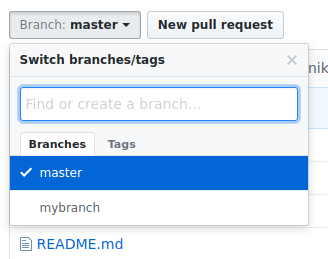
\includegraphics[width=0.5\linewidth]{../images/png/selbranch}
			\caption[Pilih Branch]{\small{Pilih cabang/branch}}
		\end{figure}
%=============================================================================
\newpage
		\item Klik tombol \textbf{New Pull Request} pada halaman repositori.
		\begin{figure}[h!]
			\centering
			\captionsetup{justification=centering}
			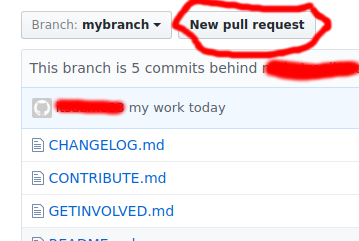
\includegraphics[width=0.5\linewidth]{../images/png/pullreq}
			\caption[Pull Request]{\small{Pull Request}}
		\end{figure}
	
		\item Setelah muncul halaman \textit{pull request}, anda dapat me-review kembali sebelum benar-benar menerbitkan \textit{pull request}.
		 \begin{figure}[h!]
		 	\centering
		 	\captionsetup{justification=centering}
		 	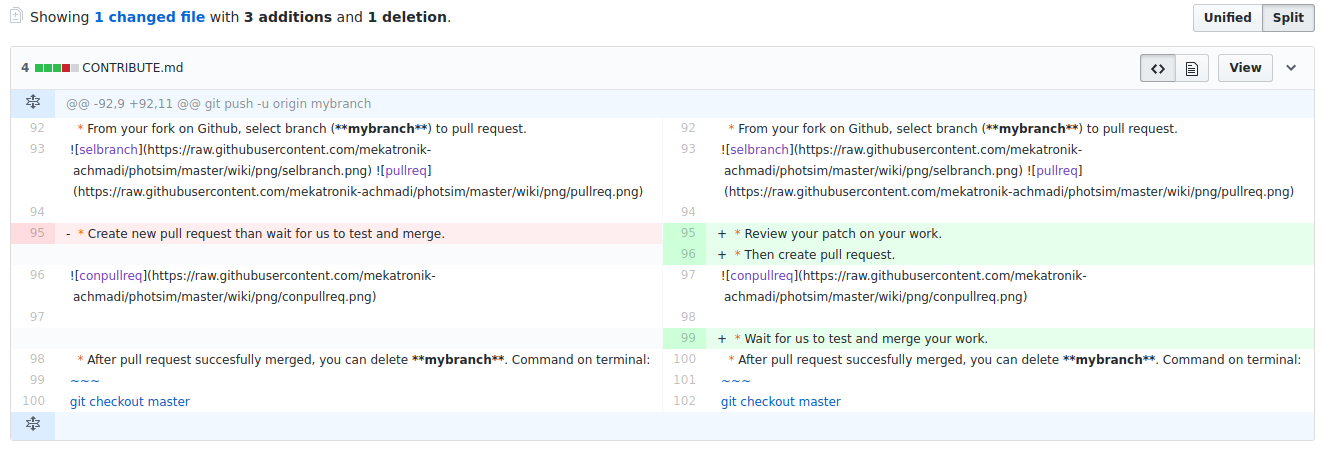
\includegraphics[width=1\linewidth]{../images/png/patchreview}
		 	\caption[Review Patch]{\small{Review Patch}}
		 \end{figure}
	 
	 	\item Terakhir, anda dapat menerbitkan pull request dengan klik tombol \textbf{Create pull request}.
	 	
	 	\begin{figure}[h!]
	 		\centering
	 		\captionsetup{justification=centering}
	 		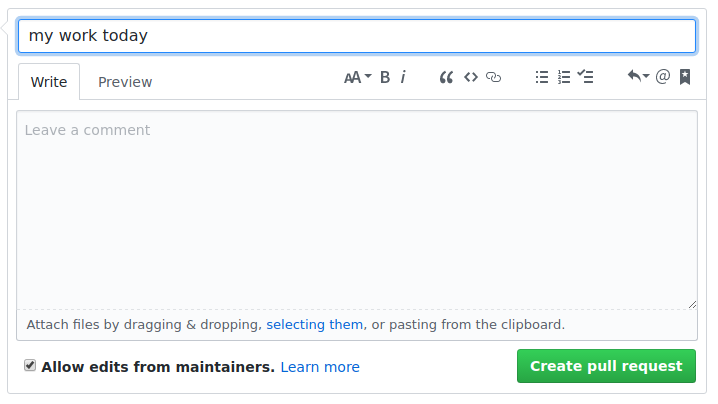
\includegraphics[width=0.8\linewidth]{../images/png/conpullreq}
	 		\caption[Issue Pull Request]{\small{Issue Pull Request}}
	 	\end{figure}
		  
	\end{itemize}

	\subsubsection{Hapus Branch/Cabang}
	
	Tahapan terakhir adalah anda dapat menghapus cabang/branch yang sebelumnya anda kerjakan.
	Perlu diperhatikan, sebaiknya anda menghapus cabang/branch jika memang \textit{pull-request} telah diterima dan di-\textit{merge} oleh maintainer.
	Jika \textit{pull-request} telah diterima, maka akun Github anda akan menerima pesan:
	 
	\begin{figure}[h!]
		\centering
		\captionsetup{justification=centering}
		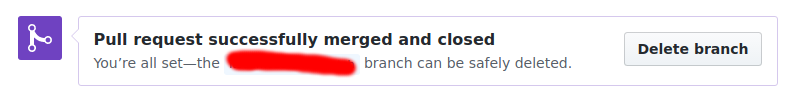
\includegraphics[width=0.8\linewidth]{../images/png/mergeok}
		\caption[Pull Request Accepted]{\small{Pull Request Accepted}}
	\end{figure}

	Jika anda telah menerima pesan tersebut, maka anda dapat hapus cabang/branch tempat anda bekerja sebelumnya.
	Berikut langkah mudah menghapus cabang/branch yang disini dicontohkan dengan nama \textbf{mybranch}:
	
	\begin{itemize}
		\item Buka Git Bash (Windows) atau Bash Shell (Linux) pada direktori/folder repositori.
		
		\item Pindah branch ke yang \textbf{master} atau branch utama
		\begin{minted}[frame=lines,fontsize=\footnotesize]{bash}
git checkout master
		\end{minted}
		
		\item Hapus branch \textbf{mybranch}
		\begin{minted}[frame=lines,fontsize=\footnotesize]{bash}
git branch -d mybranch
		\end{minted}
		
		\item Cek semua branch yang masih ada, pastikan tidak ada \textbf{mybranch}
		\begin{minted}[frame=lines,fontsize=\footnotesize]{bash}
git show-branch -a
		\end{minted}
		
		\item Terakhir hapus juga branch \textbf{mybranch} yang ada di Github anda
		\begin{minted}[frame=lines,fontsize=\footnotesize]{bash}
git push origin --delete mybranch
		\end{minted}
		
	\end{itemize}

	\subsection{Maintainer}
	
	Pada bagian ini, akan dibahas mengenai tugas akun \textit{maintainer} dari suatu proyek repositori di Github.
	Tugas utama maintainer adalah:
	
	\begin{itemize}
		\item Menerima pull-request
		\item Menguji pull-request
		\item Me-\textit{merge} pull-request ke cabang utama (\textbf{master})
		\item Ikut berkontribusi mengembangkan proyek
	\end{itemize} 

	Pada pembahasan ini hanya akan difokuskan pada bagaimana \textit{merge} pull request.

%=============================================================================
\newpage
	Pada tahap ini, dilakukan empat langkah utama, yaitu:
	\begin{itemize}
		\item Mengambil \textit{Pull Request}
		\item Menguji \textit{Pull Request}
		\item Merge \textit{Pull Request}
		\item Hapus Branch/Cabang 
	\end{itemize}

	Untuk pembahasan \textit{merging} disini, pada dasarnya dapat dilakukan pada repositori di Github menggunakan webbrowser.
	Namun untuk pembahasan ini dilakukan melalui lokal komputer/laptop dulu kemudian di \textit{push} ke Github.

	\subsubsection{Mengambil \textit{Pull Request}}
	
	Pada tahapan ini, anda sebagai \textit{maintainer} menarik pull-request yang ada di Github anda ke lokal komputer/laptop.
	Berikut adalah langkah-langkahnya:
	
	\begin{itemize}
		\item Buka Git Bash (Windows) atau Bash Shell (Linux) pada direktori/folder repositori.
		
		\item Pindah branch ke yang \textbf{master} atau branch utama
		\begin{minted}[frame=lines,fontsize=\footnotesize]{bash}
git checkout master
		\end{minted}
		
		\item Buat branch/cabang baru kemudian pindah ke branch tersebut.
		Sebagai contoh \textit{pull request} yang anda dapat memiliki: 
		\begin{itemize}
			\item user name: \textbf{friends}
			\item repositori proyek: \textbf{photsim}
			\item cabang repositori: \textbf{mybranch}
		\end{itemize}
		\begin{minted}[frame=lines,fontsize=\footnotesize]{bash}
git branch friends-mybranch
git checkout friends-mybranch
		\end{minted}
		
		\item kemudian anda \textit{pull} atau tarik \textit{pull request} yang anda dapat ke lokal pada branch ini
		\begin{minted}[frame=lines,fontsize=\footnotesize]{bash}
git pull https://github.com/friends/photsim.git mybranch
		\end{minted}
		
	\end{itemize}
	
	\subsubsection{Menguji \textit{Pull Request}}
	
	Selanjutnya, bila diperlukan anda dapat mereview ulang atau bahkan menguji \textit{patch} dari \textit{pull request} yang anda tarik sebelumnya.
	Perlu diingat bahwa cabang/branch yang sedang anda review/uji adalah \textbf{mybranch}, bukan \textbf{master}.

%=============================================================================
\newpage
	\subsubsection{Merge \textit{Pull Request}}
	
	Selanjutnya setelah \textit{patch} siap di merge, maka anda tinggal kembali ke branch/cabang \textbf{master} dan menyatukan (\textit{merge}) dengan branch anda sebelumnya
	Berikut langkah merge:
	
	\begin{itemize}
		\item Buka Git Bash (Windows) atau Bash Shell (Linux) pada direktori/folder repositori.
		
		\item Pindah kembali ke branch/cabang \textbf{master}.
		\begin{minted}[frame=lines,fontsize=\footnotesize]{bash}
git checkout master
		\end{minted} 
		
		\item Satukan atau \textit{merge} branch \textbf{friends-mybranch} ke \textbf{master}
		\begin{minted}[frame=lines,fontsize=\footnotesize]{bash}
git merge -m "my friend works" friends-mybranch
		\end{minted}

		\item \textit{Push} atau upload ke akun Github anda sebagai \textit{maintainer}.
		\begin{minted}[frame=lines,fontsize=\footnotesize]{bash}
git push origin master
		\end{minted}
	\end{itemize} 
	
	\subsubsection{Hapus Branch/Cabang}
	
	Tahapan terakhir adalah anda dapat menghapus cabang/branch lokal yang sebelumnya anda \textit{merge} ke branch master.
	Langkah untuk hapus branch:
	
	\begin{itemize}
		\item Buka Git Bash (Windows) atau Bash Shell (Linux) pada direktori/folder repositori.
		
		\item Pindah branch ke yang \textbf{master} atau branch utama
		\begin{minted}[frame=lines,fontsize=\footnotesize]{bash}
git checkout master
		\end{minted}
		
		\item Hapus branch \textbf{friends-mybranch}
		\begin{minted}[frame=lines,fontsize=\footnotesize]{bash}
git branch -d friends-mybranch
		\end{minted}
		
		\item Cek semua branch yang masih ada, pastikan tidak ada \textbf{friends-mybranch}
		\begin{minted}[frame=lines,fontsize=\footnotesize]{bash}
git show-branch -a
		\end{minted}
	\end{itemize}

	\subsection{Info Graphic}
	
	Seluruh metode Git Kolaborasi dapat diringkas menjadi info graphic pada halaman selanjutnya.

%=============================================================================
\newpage

	

%=============================================================================
%\newpage
%\thispagestyle{plain}
%\mbox{}

%=============================================================================
% Daftar Pustaka
%\newpage
%
%	\section{Daftar Pustaka}
%	
%	\begin{center}
%		\textbf{Daftar Pustaka}
%	\end{center}
%	
%	\bibliographystyle{IEEEtran}
%	\bibliography{/home/achmadi/Documents/BibTex/library.bib}
%	\bibliography{/home/fotoniks/Mendeley_BibTex/library.bib}

%=============================================================================
	
\end{document}
